%-------------------------------------------------------------------------------
%-------------------------------------------------------------------------------
%-------------------------------------------------------------------------------
\chapter{Modélisation d'un amortisseur}
%-------------------------------------------------------------------------------
%-------------------------------------------------------------------------------
\thispagestyle{empty}
%-------------------------------------------------------------------------------
\section{Présentation}
%-------------------------------------------------------------------------------
%-------------------------------------------------------------------------------
%-------------------------------------------------------------------------------
Le laboratoire de sciences industrielles dispose du matériel qui permet d'étudier une suspension de moto avec la possibilité d'effectuer des mesures.

\begin{center}
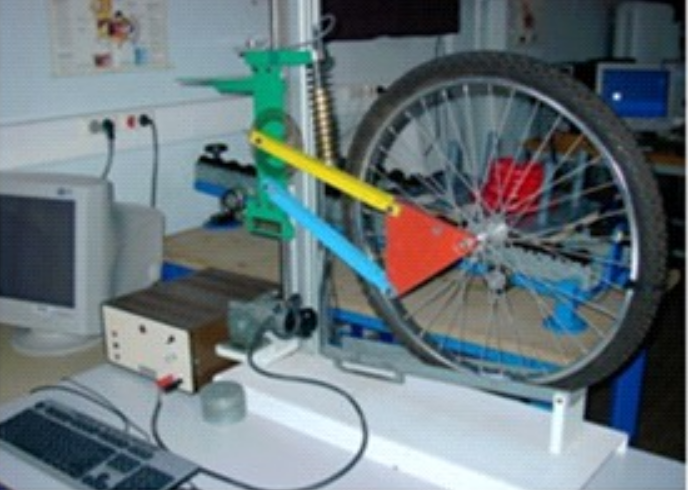
\includegraphics[scale=0.4]{Images/14_dispositif}
\end{center}

Lors de la manipulation un capteur (un accéléromètre) calcule les accélérations d'un point de la partie mobile et enregistre celles-ci dans un fichier texte.

On souhaite traiter ce fichier afin de corréler l'expérience avec un modèle de connaissance du type oscillant amorti.

\medskip
Il s'agit donc d'étudier le mouvement vertical oscillant amorti d'un solide en translation verticale dans un champ gravitationnel vertical dirigé vers le bas.

 Le solide est guidé par une liaison de direction verticale possédant :
\begin{itemize}
%--------------------------------------------------------------------------
\item une raideur qui crée une force, en $[N]$, proportionnelle au déplacement vertical relatif par rapport à la position d'équilibre en $[m]$ et qui s'oppose au déplacement,
%--------------------------------------------------------------------------
\item un amortissement visqueux qui crée une force verticale en $[N]$ qui s'oppose à la vitesse de déplacement relative entre le solide et la référence en $[m \cdot s^{-1}]$.
%--------------------------------------------------------------------------
\end{itemize}
%--------------------------------------------------------------------------
%--------------------------------------------------------------------------
\subsection{Création du fichier}%
%--------------------------------------------------------------------------
%--------------------------------------------------------------------------
Le fichier est créé selon le protocole suivant.
%--------------------------------------------------------------------------
\begin{itemize}
\item On part de la position d'équilibre statique du système.
\item On déplace manuellement vers le bas de $100${\small \it mm} le châssis de la moto.
\item On lance une acquisition pour $6s$ avec une fréquence d'échantillonnage de $200Hz$.
\item On lâche le châssis sans condition initiale de vitesse.
\item On sauvegarde le fichier relatif à l'expérience sous le nom \texttt{moto1.txt} en demandant une indexation des points.
\end{itemize}
%--------------------------------------------------------------------------
\begin{itemize}
  \item Le fichier \type{moto.txt} est une suite de caractères générée par le logiciel d'acquisition. 
%--------------------------------------------------------------------------
  \item Il comporte $1200$ lignes car l'acquisition se fait à $200Hz$ pour une acquisition de $6$ secondes.
%--------------------------------------------------------------------------
  \item Chaque ligne est l'enregistrement de 4 nombres :
  
  \medskip
\begin{center}
\begin{tabular}{rrrr}
% \textbf{Colonne 1}& \textbf{Colonne 2}&\textbf{Colonne 3}&\textbf{Colonne 4}\\
% \hline
\type{1} & \type{+0.0000000} & \type{+7.3876953} & \type{+1.9042969}\\
\type{2} & \type{-0.0048828} & \type{+7.3925781} & \type{+1.8994141}\\
\type{3} & \type{-0.0097656} & \type{+7.3974609} & \type{+1.8994141}\\
\dots&\dots&\dots&\dots\\
\type{1200} & \type{-0.0048828} & \type{+7.3925781} & \type{+1.5283203}\\
\end{tabular}
\end{center}
  
  \medskip
%--------------------------------------------------------------------------
\item La première colonne donne le numéro de la mesure, ici de 1 à 1200.
%--------------------------------------------------------------------------
\item Les trois dernières colonnes correspondent aux mesures de l'accéléromètre, ce sont des tensions qui dépendent linéairement des composantes de l'accélération dans une base orthonormée : à l'équilibre, elles mesurent l'accélération de la pesanteur. La composante verticale est écrite dans la deuxième coordonnée, c'est-à-dire la troisième colonne. C'est cette mesure que nous étudierons.
%--------------------------------------------------------------------------
\item Dans le fichier, chaque ligne est donc composée de quatre éléments.

Ces éléments sont séparés par des caractères de tabulation, \type{"$\backslash$t"}.

Chaque ligne est terminée par un caractère de changement de ligne \type{"$\backslash$n"}.
%--------------------------------------------------------------------------
\end{itemize}

On peut ouvrir le fichier dans un éditeur pour en lire la structure. 

Dans un éditeur classique les tabulations et les retours à la lignes seront traduits et on obtient un alignement vertical comme dans l'exemple ci-dessus.
%--------------------------------------------------------------------------
%--------------------------------------------------------------------------
\subsection{Objectifs}
%--------------------------------------------------------------------------
%--------------------------------------------------------------------------
\begin{enumerate}
  \item Lire le fichier texte \texttt{moto1.txt}.
  \item Convertir le fichier lu en une structure de données utilisable par python.
  \item Transformer ces données pour obtenir une représentation de la vitesse et de la position de l'accéléromètre.
  \item Rechercher les grandeurs caractéristiques associées à un modèle mécanique permettant son identification.
\end{enumerate}
%--------------------------------------------------------------------------
%--------------------------------------------------------------------------
\newpage
%--------------------------------------------------------------------------
\section{Lecture du fichier}
%--------------------------------------------------------------------------
%--------------------------------------------------------------------------
%--------------------------------------------------------------------------
Pour utiliser un fichier on doit ouvrir une connexion avec celui-ci par l'instruction \type{open}. Celle-ci a deux arguments : le nom du fichier (une chaîne de caractères) et le type qui peut être \type{"r"} pour la lecture, \type{"w"} pour l'écriture d'un nouveau fichier et \type{"a"} pour l'ajout à un fichier existant. 

On peut importer le fichier 
%--------------------------------------------------------------------------
\begin{itemize}
\item comme une grande chaîne de caractères : \type{read}
\item comme une liste de lignes : \type{readlines}
\item ligne à ligne : \type{readline}
\end{itemize}
%--------------------------------------------------------------------------
Une ligne est une portion du fichier délimitée par le caractère de retour à la ligne \type{"$\backslash$n"}, ce caractère est conservé en fin de ligne.

On obtient donc la liste des lignes du fichier d'acquisition avec
%--------------------------------------------------------------------------
\begin{lstlisting}
## Importations
nom = 'moto.txt'
fichier = open(nom, 'r')
listeBrute = fichier.readlines()
fichier.close()
\end{lstlisting}
%--------------------------------------------------------------------------
On rappelle l'importance de fermer la communication : \type{fichier.close()}.

\medskip

Le fichier est lu par python dans le répertoire de travail.

Python contient un module, \type{os}, qui permet d'interagir avec le système de fichiers. 
%--------------------------------------------------------------------------
\begin{lstlisting}
import os 
\end{lstlisting}
%--------------------------------------------------------------------------

On peut connaître le répertoire de travail avec \type{os.getcwd()}.

On peut se déplacer dans l'arborescence du disque avec la fonction \type{os.chdir} ; la méthode la plus simple pour l'utiliser est de donner le nom complet du répertoire comme argument. Cela change le répertoire de travail.

%--------------------------------------------------------------------------
\begin{lstlisting}
## Importations
import os 

os.chdir("/home/profs/detrez.eric/Travail/2018-2019") # Linux
# os.chdir("H://Travail//2018-2019") # Sous Windows
\end{lstlisting}
%--------------------------------------------------------------------------
On notera le dédoublement du séparateur \type{"//"} sous Windows.

\medskip

On peut aussi donner le chemin complet d'accès au fichier comme paramètre.
%--------------------------------------------------------------------------
%--------------------------------------------------------------------------
\begin{Exercise}\it Importer, comme indiqu" ci-dessus, les lignes du fichiers \type{moto.txt}.
\end{Exercise}
%--------------------------------------------------------------------------
%--------------------------------------------------------------------------
\begin{Answer}
\end{Answer}
%--------------------------------------------------------------------------
%--------------------------------------------------------------------------
On peut voir la structure non traduite des lignes dans la console ; la fonction \type{print} interprète les caractères spéciaux donc produit un affichage différent.
%-------------------------------------------------------------------------------
\begin{lstlisting}
>>> listeBrute[55]
'        56\t-0.0097656\t+7.3974609\t+1.8945313\n'

>>> print(listeBrute[55])
        56	-0.0097656	+7.3974609	+1.8945313
\end{lstlisting}
%--------------------------------------------------------------------------
%-------------------------------------------------------------------------------
\newpage
%--------------------------------------------------------------------------
\section{Traitement initial}
%--------------------------------------------------------------------------
%--------------------------------------------------------------------------
%--------------------------------------------------------------------------
\subsection{Conversion en nombres}
%--------------------------------------------------------------------------
%--------------------------------------------------------------------------
On veut maintenant convertir les chaînes de caractères obtenues en données numériques.

On pourra utiliser
\begin{itemize}
  \item une extraction \type{ch[:-1]} pour enlever le dernier caractère (\type{"$\backslash$n"})
  \item la méthode \type{split(c)} qui transforme une chaîne de caractères en une liste de chaînes de caractères qui sont les morceaux découpé par le paramètre. Par exemple
\begin{lstlisting}
>>> ch = "anticonstitutionnellement"
>>> ch.split('t')
['an', 'icons', 'i', 'u', 'ionnellemen', '']
>>> ch.split('ti')
['an', 'cons', 'tu', 'onnellement']
>>> ch.split('n')
['a', 'tico', 'stitutio', '', 'elleme', 't']
\end{lstlisting}
\item la fonction de conversion de type, ici \type{float}, pour transformer une chaîne en flottant.
\end{itemize}

%--------------------------------------------------------------------------
%--------------------------------------------------------------------------
\begin{Exercise}\it Écrire une fonction \type{traduction(ch)} qui transforme une chaîne de caractères semblable aux lignes du fichiers en une liste de nombre.
\end{Exercise}
%--------------------------------------------------------------------------
%--------------------------------------------------------------------------
\begin{Answer}
\begin{lstlisting}
def traduction(ch):
    """Entrée : une chaîne de caractères représentant
                une suite de nombres séparés par des tabulations
                et terminant par '\n'
       Sortie : la liste de ces nombres"""
    ch1 = ch[:-1] # On enlève le caractère '\n' final
    l1 = ch1.split('\t') # On découpe
    l2 = [] 
    n = len(l1)
    for i in range(n):          # Les éléments 
        l2.append(float(l1[i])) # sont sont convertis en flottants
    return l2
\end{lstlisting}
On peut aussi faire le travail à la main.
\begin{lstlisting}
def traduction(ch):
    """Entrée : une chaîne de caractères représentant
                une suite de nombres séparés par des tabulations
                et terminant par '\n'
       Sortie : la liste de ces nombres"""
    l = []
    morceau = ''
    for car in ch: # On lit les caractères
        if car == '\t' or car == '\n': # fin d'un morceau
            l.append(float(morceau)) # on covertir en nombre
            morceau = '' # on re-initialise le morceau
        else:
            morceau = morceau + car # on ajoute le caractère
    return l                
\end{lstlisting}
\end{Answer}
%--------------------------------------------------------------------------
%--------------------------------------------------------------------------
\begin{Exercise}\label{qu:liste}\it Écrire les instructions (dans la partie principale) qui permettent de traduire \type{listeBrute} en une liste \type{liste} dont les éléments sont des listes de 4 nombres.
\end{Exercise}
%--------------------------------------------------------------------------
\begin{Answer}
\begin{lstlisting}
liste = []
n = len(listeBrute)
for i in range(n):
    liste.append(traduction(listeBrute[i]))
\end{lstlisting}
ou \type{liste = [traduction(ch) for ch in listeBrute]}
\newpage
\end{Answer}
%--------------------------------------------------------------------------
%--------------------------------------------------------------------------
Le premier élément de la liste devra donc être \type{[1.0, 0.0000000, 7.3876953, 1.9042969]}.
%--------------------------------------------------------------------------
%--------------------------------------------------------------------------
\subsection{Extraction des colonnes}
%--------------------------------------------------------------------------
%--------------------------------------------------------------------------
\begin{Exercise}\it Écrire une fonction \type{extraire(k,liste)} où $k$ est un entier et \type{liste} est une liste dont les éléments sont des listes de longueur $k$ au moins et qui renvoie la liste des $k$-ièmes composantes.

\type{extraire(2, [[1, 2, 3], [4, 5, 6]])} doit renvoyer \type{[2, 5]}
\end{Exercise}
{\bf N.B. La $k$-ième composante correspond à l'indice $k-1$.}
%--------------------------------------------------------------------------
\begin{Answer}
\begin{lstlisting}
def extraire(k,liste):
    """Entrée : un entier et une liste
       Requis : les éléments de la liste sont des listes 
                de longueur au moins k
       Sortie : la liste des k-ièmes composantes"""
    resultat  = []
    for l in liste:
        resultat.append(l[k-1])
    return resultat
\end{lstlisting}
On peut aussi utiliser les raccourcis python
\begin{lstlisting}
def extraire(k,liste):
    return [l[k-1] for l in liste]
\end{lstlisting}
\end{Answer}
%--------------------------------------------------------------------------
%--------------------------------------------------------------------------
\medskip

On peut maintenant visualiser les différentes colonnes.

On utilise pour cela le module \type{matplotlib}
%--------------------------------------------------------------------------
\begin{lstlisting}
import matplotlib.pyplot as plt 
\end{lstlisting}
%--------------------------------------------------------------------------
Le nom raccourci \type{plt} est usuel.

On affiche une liste de nombre, \type{X}, par
%--------------------------------------------------------------------------
\begin{lstlisting}
plt.plot(X) 
plt.show()
\end{lstlisting}
%--------------------------------------------------------------------------
%--------------------------------------------------------------------------
\begin{Exercise}\it Afficher les valeurs des 4 colonnes ; commentez.
\end{Exercise}
%--------------------------------------------------------------------------
\begin{Answer}
\begin{itemize}
  \item Pour la première colonne les valeurs sont affines par rapport à l'indice.
  \item La deuxième colonne semble être du bruit
  \item La troisième et la quatrième colonnes montrent des oscillations, un peu bruitées. 
\end{itemize}
\end{Answer}
%--------------------------------------------------------------------------
%--------------------------------------------------------------------------
\newpage
%--------------------------------------------------------------------------
\section{Traitement des listes}
%--------------------------------------------------------------------------
%--------------------------------------------------------------------------
%--------------------------------------------------------------------------
Dans cette section on se propose 
\begin{itemize}
  \item de déterminer l'origine temporelle des variations,
  \item de convertir les résultats signifiants en unité connues,
  \item de calculer puis retirer l'accélération gravitationnelle,
  \item de calculer les vitesses puis les déplacement à partir de l'accélération.
\end{itemize}  

On définit, après les instructions de la {\bf question \ref{qu:liste}}, les listes particulières :
\begin{lstlisting}
tempsBrut = extraire(1, liste)
accBrute = extraire(3, liste)
\end{lstlisting}
%--------------------------------------------------------------------------
%--------------------------------------------------------------------------
\subsection{Origine et échelle du temps}
%--------------------------------------------------------------------------
%--------------------------------------------------------------------------
Le tracé de \type{accBrute} montre que l'accélération n'a pas varié immédiatement, il s'est passé du temps entre le déclenchement de la lecture des données et le lâcher de la roue. Pour déterminer l'origine du mouvement on va déterminer l'indice en lequel l'accélération a comment à varier au-delà des variations aléatoires.
%--------------------------------------------------------------------------
%--------------------------------------------------------------------------
\begin{Exercise}\it 
Écrire une fonction \type{rechZero(liste, ecart)} qui recherche le premier indice pour lequel la valeur de la liste s'écarte d'au moins \type{ecart} de la valeur initiale. On veut donc le premier indice $i$ tel que \type{abs(liste[i] - liste[0] >= ecart}.
\end{Exercise}
%--------------------------------------------------------------------------
\begin{Answer} On choisit de renvoyer la longueur de la liste si elle ne diffère jamais de plus d'écart depuis sa position initiale.
\begin{lstlisting}
def rechZero(liste,ecart):
    """Entrée : une liste et un nombre
       Sortie : le premier indice en lequel
                la liste diffère de liste[0] 
                d'au moins ecart"""
    init = liste[0]
    n = len(liste)
    for i in range(n):
        if abs(liste[i] - init) >= ecart:
            return(i)
    return n
\end{lstlisting}
\end{Answer}
%--------------------------------------------------------------------------
%--------------------------------------------------------------------------
\medskip

On choisit dans la suite un écart assez petit\footnote{Mais pas trop petit pour éviter les variations aléatoires.} pour déterminer l'origine temporelle. On ajoutera, par exemple, l'instruction suivante dans la partie principale.
\begin{lstlisting}
i0 = rechZero(accBrute, 1e-2) - 1
\end{lstlisting}
On a retranché 1 car le premier écart correspond à la deuxième mesure du mouvement.
\medskip
Avec la fréquence d'échantillonnage, on connaît le temps entre deux mesures : $\Delta t=\frac 1f=0.005\, s$. 

On notera \type{Delta\_t} une variable qui prend la valeur $\Delta t$ dans la suite.
%--------------------------------------------------------------------------
%--------------------------------------------------------------------------
\begin{Exercise}\it 
Écrire les instructions (dans la partie principale) qui calculent la liste des temps en secondes, notée \type{temps}, en commençant avec $t=0$ pour l'origine du phénomène (le point d'indice \type{i0}). 

La liste sera plus courte que la liste originale.
\end{Exercise}
%--------------------------------------------------------------------------
\begin{Answer}
\begin{lstlisting}
f = 200
Delta_t = 1/f
x0 = tempsBrut[i0]
n = len(tempsBrut)
temps = []
for i in range(i0, n):
    x = tempsBrut[i]
    t = (x-x0)*Delta_t
    temps.append(t)
\end{lstlisting}

La boucle peut être remplacée par \type{temps = [(x-x0)*Delta\_t for x in tempsBrut[i0:]]}
\newpage
\end{Answer}
%--------------------------------------------------------------------------
%--------------------------------------------------------------------------
\subsection{Échelle des accélérations}
%--------------------------------------------------------------------------
%--------------------------------------------------------------------------
Lorsqu'il est au repos, c'est-à-dire pour les indices de 0 à $i_0$, le dispositif ne subit que l'accélération de la pesanteur. On considère donc la moyenne des valeurs de \type{accBrute} pour ces indices comme valeur de la mesure de cette accélération de la pesanteur. On rappelle que cette mesure est donnée en Volts, on devra la convertir en $m\cdot s^{-2}$.
%--------------------------------------------------------------------------
%--------------------------------------------------------------------------
\begin{Exercise}\it Écrire une fonction \type{moy(liste)} qui calcule la valeur moyenne de la liste.

En déduire une valeur, $V_g$, de la mesure de $g$ fournie par l'accéléromètre (dans la partie principale).
\end{Exercise}
%--------------------------------------------------------------------------
\begin{Answer}
\begin{lstlisting}
def moy(liste):
    """Entrée : une liste non vide
       Sortie : la moyenne des termes"""
    n = len(liste) 
    som = 0 
    for i in range(n):
        som = som + liste[i] 
    return som/n
\end{lstlisting}

\begin{lstlisting}
Vg = moy(accBrute[0:i0])
\end{lstlisting}
\end{Answer}
%--------------------------------------------------------------------------
%--------------------------------------------------------------------------
\medskip

L'accéléromètre mesure l'accélération $a$ (sous la forme d'une tension $V$) dans le référentiel terrestre.

On a mesuré la tension $V_0= 4,8291 V$ en l'absence de toute accélération (même gravitationnelle) et on admet que la mesure de l'accélération en $m\cdot s^{-2}$, $a$, s'obtient à partir de la tension $V$ de l'accéléromètre par une formule $a = \alpha V+\beta$.

%--------------------------------------------------------------------------
%--------------------------------------------------------------------------
\begin{Exercise}\it 
Après avoit définie les variables \type{g = 9.81} et \type{V0 = 4.8291}, écrire, dans la partie principale, les instructions permettant de calculer les variables \type{alpha} et \type{beta} prenant les valeurs des coefficients de la formule ci-dessus.
\end{Exercise}
%--------------------------------------------------------------------------
\begin{Answer} On a $\alpha V_0 + \beta = 0$ et $\alpha V_g + \beta = g$
\begin{lstlisting}
v0 = 4.8291
g = 9.81

alpha = g/(Vg - V0)
beta = -alpha*V0
\end{lstlisting}
\end{Answer}
%--------------------------------------------------------------------------
%--------------------------------------------------------------------------

L'accélération du dispositif isolé est l'accélération mesurée à laquelle on retire $g$.
%--------------------------------------------------------------------------
%--------------------------------------------------------------------------
\begin{Exercise}\it 
Écrire les instructions (dans la partie principale) qui calculent la liste des accélérations du dispositif en $m/s^2$, notée \type{acc}, en commençant avec $t=0$ c'est-à-dire à partir de l'indice $i_0$.

\type{acc} sera donc de même longueur que la liste \type{temps}.
\end{Exercise}
%--------------------------------------------------------------------------
\begin{Answer}
\begin{lstlisting}
acc = []
for i in range(i0, n):
    aV = accBrute[i]
    a = alpha*aV + beta - g
    acc.append(a)
\end{lstlisting}

ou, en utilisant la définition de listes par compréhension,
\begin{lstlisting}
acc = [alpha*aV + beta - g for aV in accBrute[i0:]]
\end{lstlisting}
\end{Answer}
%--------------------------------------------------------------------------
%--------------------------------------------------------------------------
\medskip

On a maintenant une liste dont les valeurs sont les temps, régulièrement espacés, en lesquels le système a mesuré une accélération. Si on note $t_i$ la valeur de \type{liste[i]} alors la valeur \type{acc[i]} est la valeur de l'accélération au temps $t_i$.

On peut alors représenter cette fonction accélération en fonction du temps.
%--------------------------------------------------------------------------
\begin{lstlisting}
plt.plot(temps,acc)
plt.show()
\end{lstlisting}
%--------------------------------------------------------------------------
\type{matplotlib} permet d'ajouter beaucoup de personnalisations aux graphes.
%--------------------------------------------------------------------------
\begin{lstlisting}
plt.title("Accélération") # Ajout d'un titre 		
plt.xlabel("Temps en secondes") # Légende des abscisses		
plt.ylabel("Accélération en m/s^2") # Légende des ordonnées			
plt.grid(True) # Ajout d'une grille 
plt.plot(temps,acc,
         color="magenta", # couleur de la ligne
         linewidth=2.5,   # épaisseur de la ligne
         linestyle="-",   # type de ligne
         label="Accélération") # nom de la fonction tracée
plt.legend() # écriture du "label"
plt.show()
\end{lstlisting}
%--------------------------------------------------------------------------
%--------------------------------------------------------------------------
\subsection{Vitesses et positions}
%--------------------------------------------------------------------------
%--------------------------------------------------------------------------
On cherche ensuite à évaluer les vitesses et les positions aux temps $t_i$.

Si on connaît une fonction en des points $t_0$, $t_1$, \dots, $t_p$ et si $t_i$ et $t_{i+1}$ sont suffisamment proches on peut approcher la variation de ses primitives (l'intégrale) par la formule du rectangle : $\displaystyle F(t_{i+1}) - F(t_i)\sim {t_{i+1} - t_i}. f(t_i)$.

On peut alors calculer les valeurs de $F$ de proche en proche à partir d'une valeur initiale $F(t_0)$.

Ici $t_{i+1} - t_i$ est constante, c'est $\Delta t$
%--------------------------------------------------------------------------
%--------------------------------------------------------------------------
\begin{Exercise}\it 
Écrire une fonction \type{primitive(listeFn, dt, y0)} où \type{listeFn} est une liste représentant les valeurs de $f(t_i)$, \type{dt} est le pas de temps et \type{valeurInit} est la valeur initiale de la primitive, $F(t_0)$ et qui renvoie une liste, de même longueur que \type{listeDer}, contenant des valeurs approchées de $F(t_i)$.
\end{Exercise}
%--------------------------------------------------------------------------
\begin{Answer}
\begin{lstlisting}
def primitive(listeFn, dt, y0):
    """Entrée : une liste de nombres et deux nombres
       Sortie : la liste des valeurs des primitives"""
    prim = [0]*n
    prim[0] = y0
    n = len(listeFn)
    for i in range(n-1): # il reste n-1 valeurs à calculer
        prim[i+1] = prim[i] + dt*listeFn[i]
    return prim
\end{lstlisting}
\end{Answer}
%--------------------------------------------------------------------------
On remarque qu'on n'utilise pas la dernière valeur de \type{listeFonction}.

\medskip

%--------------------------------------------------------------------------
%--------------------------------------------------------------------------
\begin{Exercise}\it Calculer et tracer le graphe des vitesses et des positions.

La vitesse initiale est 0 m.s$^{-1}$, la position initiale est -0,10 m.
\end{Exercise}
%--------------------------------------------------------------------------
\begin{Answer}
\begin{lstlisting}
vit = primitive(acc, Delta_t, 0)
pos = primitive(vit, Delta_t, -0.1)

plt.subplot(3,1,1)          
plt.title("Accélération") 
plt.grid(True)
plt.plot(temps,acc) 
plt.subplot(3,1,2)          
plt.title("Vitesse") 
plt.grid(True)
plt.plot(temps,vit)
plt.subplot(3,1,3)          
plt.title("Position") 
plt.grid(True)
plt.plot(temps,pos)
plt.show()
\end{lstlisting}
\end{Answer}
%--------------------------------------------------------------------------
%--------------------------------------------------------------------------
On peut voir que la position ne reste pas stable à la valeur 0 à la fin des oscillations. Si on prend pour $V_g$ la moyenne des valeurs de \type{accbrute} sur toute la suite, le résultat sera meilleur.
%--------------------------------------------------------------------------
%--------------------------------------------------------------------------
\begin{Exercise}\it 
Enregistrer la suite des valeurs des temps et des positions dans un fichier \type{moto1.txt}.
\end{Exercise}
%--------------------------------------------------------------------------
\begin{Answer}
\begin{lstlisting}
fichier = open("moto1.txt", "w')
n = len(pos)
for i in range(n):
    x = str(temps[i]) + "\t" + str(pos[i]) + "\n"
    fichier.write(x)
fichier.close()
\end{lstlisting}
\end{Answer}
%--------------------------------------------------------------------------
%--------------------------------------------------------------------------
%--------------------------------------------------------------------------
\section{Compléments : identification des caractéristiques}%
%--------------------------------------------------------------------------
%--------------------------------------------------------------------------
%--------------------------------------------------------------------------
La réponse du système est identifiable à la solution de l'équation différentielle suivante :
\[\frac{1}{\omega_0^2}x''(t) + \dfrac{2\xi}{\omega_0}x'(t) + x(t) = 0\]
 
\begin{itemize}
\item où $x(t)$ est la position verticale repérée
\item $\xi$ est le coefficient d'amortissement,
\item $\omega_0$ est la pulsation propre du système
\end{itemize}

La solution telle que $x(0) = -e_0 = -0.1$ et $x'(0) = 0$ est 
\[x(t) = -e_0e^{-\xi \omega_0 t}\left( \cos(\omega t)+\frac {\xi \omega_0}{\omega}\sin(\omega t)\right)\text{ avec }\omega = \omega_0 \sqrt{1-\xi^2} \]
%--------------------------------------------------------------------------
%--------------------------------------------------------------------------
\begin{Exercise}\it 
Prouver que $\displaystyle x'(t) = \frac{e_0\omega_0}{\sqrt{1-\xi^2}}e^{-\xi \omega_0 t}\sin(\omega t)$.

En déduire les valeurs de $t$ et de $x$ aux extremums.
\end{Exercise}
%--------------------------------------------------------------------------
\begin{Answer}

$\displaystyle
x'(t) = -e_0e^{-\xi \omega_0 t}\left( -\xi \omega_0\cos(\omega t)+\frac {-\xi^2 \omega_0^2}{\omega}\sin(\omega t)
-\omega\sin(\omega t) + \xi \omega_0\cos(t)\right)$.

Or $\displaystyle \frac {\xi^2 \omega_0^2}{\omega}+\omega = \frac {\xi^2 \omega_0^2 +\omega^2}{\omega}
= \frac {\xi^2 \omega_0^2 +\omega_0^2(1-\xi^2)}{\omega}
= \frac {\omega_0^2}{\omega}
= \frac {\omega_0}{\sqrt{1-\xi^2}}$.

On voit donc que les extremums sont atteints aux temps $\displaystyle t_k = \frac{k\pi}{\omega}$ et leurs valeurs sont de la forme 
$-(-1)^ke_0 e^{-\xi \omega_0 t_k}$.
\end{Answer}
%--------------------------------------------------------------------------
%--------------------------------------------------------------------------
\medskip

On va donc calculer les valeurs du temps, $t_1$, et de la position au premier extremum après l'origine, $e_1$, on remarque que cela correspond au maximum de la courbe.

On a alors $\displaystyle \omega_0 = \frac{\pi}{t_1\sqrt{1-\xi^2}}$ et $\displaystyle \frac{\xi}{\sqrt{1-\xi^2}}=\frac {-1}\pi\ln\left(\frac{e_1}{e_0}\right)$.
%--------------------------------------------------------------------------
%--------------------------------------------------------------------------
\begin{Exercise}\it 

Écrire une fonction qui calcule l'indice (le premier) du maximum d'une liste.

En déduire les valeurs de $t_1$ et $e_1$ puis de $\xi$ et $\omega_0$.

\type{pi} et \type{log} (pour $\ln$) seront importés du module \type{math}.
\end{Exercise}
%--------------------------------------------------------------------------
\begin{Answer}
\begin{lstlisting}
def indMax(liste):
    indMax = 0
    n = len(liste)
    for k in range(n):
        if liste[k] > liste[indMax]:
            indMax =k
    return indMax
\end{lstlisting}

\begin{lstlisting}
i1 = indMax(pos)
t1 = temps[i1]
e1 = pos[i1]
q = -log(e_1/e_0)/pi
xi = q/(pi**2+q**2)**0.5
omega0 = pi/t1/(1-xi**2)**0.5
\end{lstlisting}
\newpage
\end{Answer}
%--------------------------------------------------------------------------
%--------------------------------------------------------------------------
\medskip

Voici le résultat obtenu :

\begin{center}
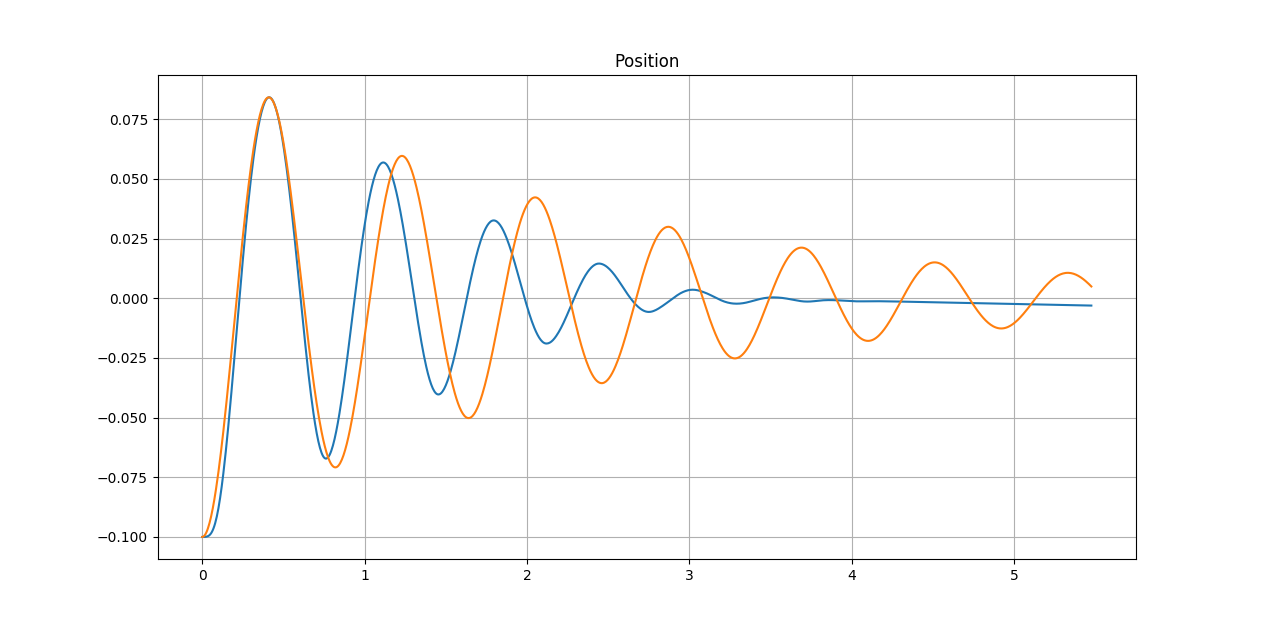
\includegraphics[scale=0.5]{Images/14_identification}
\end{center}
%--------------------------------------------------------------------------
%--------------------------------------------------------------------------
\begin{Exercise}[title={Question ouverte}]\it 

Comment améliorer les résultats ? 
\end{Exercise}
%-------------------------------------------------------------------------------
\begin{Answer}
On peut penser que le calcul de l'origine n'est pas idéal et espérer calculer les constantes à l'aide des deux premiers extremums. $t_1$ est remplacé par le temps entre les deux extremums et on calcule le quotient entre les valeurs extrémales.

On change aussi la fonction solution pour qu'elle prenne la valeur $e_1$ en $t_1$.
\begin{lstlisting}
i1 = indMax(pos)
i2 = indMinDepuis(pos, i1)
t1 = temps[i1]
t2 = temps[i2]
t = (t2-t1)
omega = pi/t
e1 = abs(pos[i1])
e2 = abs(pos[i2])
q = log(e1/e2)/pi
xi = q/(1+q**2)**0.5
omega0 = pi/t/(1-xi**2)**0.5

sol = [solution(t) for t in temps]
plt.plot(temps,pos,linestyle = "dashed", color = "black",label="Valeurs expérimentales")
plt.plot(temps, sol,color = "black",label="Valeurs théoriques")
plt.grid()
plt.legend()
plt.show()
\end{lstlisting}
C'est moins pire
\begin{center}
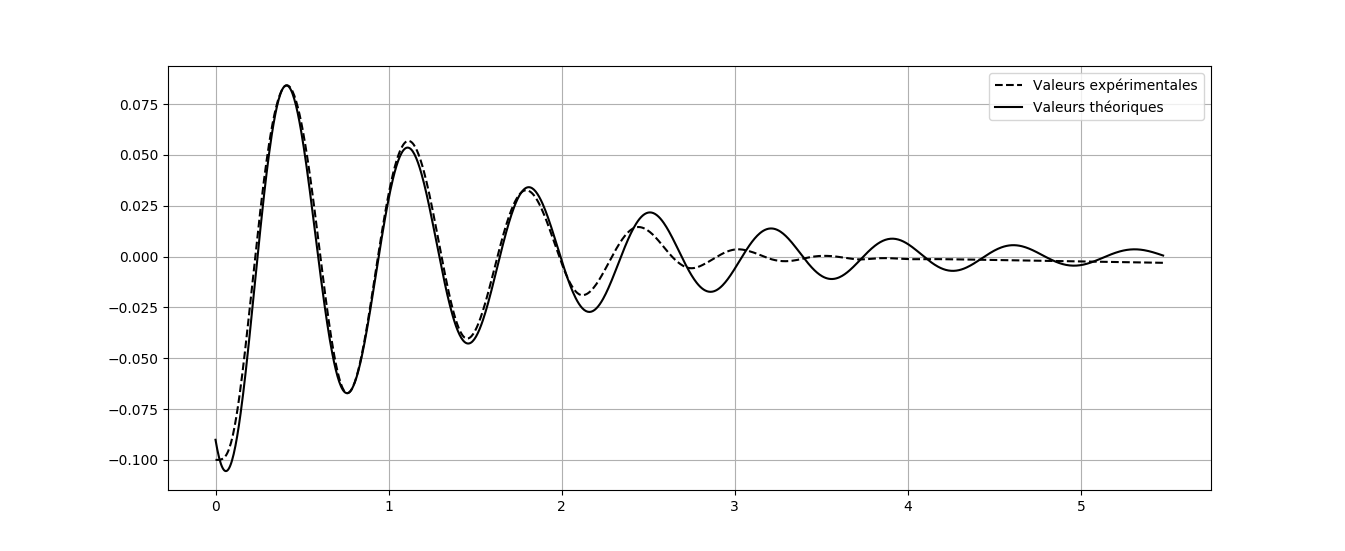
\includegraphics[scale=0.5]{Images/14_identification2}
\end{center}

\end{Answer}